\documentclass{article}
\usepackage[UTF8]{ctex}
\usepackage[tc]{titlepic}
\usepackage{titlesec}
\usepackage{amsmath}
\usepackage{cite}
\usepackage{fancyhdr}
\usepackage{booktabs}
\usepackage{graphicx}
\usepackage{hyperref}
\usepackage{geometry}
\usepackage{float}
\usepackage{xcolor}
\usepackage[section]{placeins}
\geometry{a4paper,scale=0.8}
\pagestyle{fancy}

\lhead{基于矩阵低秩分解的图像处理\\\today}
\chead{中国科学技术大学\\数学建模课程}

\rhead{Assignment 2\\ {\CTEXoptions[today=old]\today}}
\newcommand{\upcite}[1]{\textsuperscript{\cite{#1}}}

\titleformat*{\section}{\bfseries\Large}
\titleformat*{\subsection}{\bfseries\large}

\title{\bfseries 基于矩阵低秩分解的图像处理}
\author{陈鸿绪 \quad  35 \quad  PB21000224}

\begin{document}
\maketitle
\begin{abstract}
    稳健主成分分析(Robust Principal Component Analysis),是一种用于分解一个矩阵为低秩成分和稀疏成分的技术。具体来说,对于给定的矩阵M,RPCA旨在找到两个矩阵L和S,使得M=L+S,其中L是低秩的,而S是稀疏的。RPCA问题通过ALM(增广拉格朗日乘子法)转化,本次实验采用ADMM(交替方向乘子法)求解ALM。实验过程中试验了两种不同的ADMM算法,一种为传统ADMM,另外一种为不精确ADMM,传统ADMM同时拥有内循环和外循环进行迭代收敛,而不精确ADMM会通过合并两个循环进行迭代收敛。通过近似子问题求解,理论上后者比前者加速了收敛速度。在实验中,不精确算法确实比传统算法迭代收敛更快,然而结果产生了致命的问题:算法恢复出来的图像几乎和原图相差无几,噪声并没有有效剔除。所以在后续结果中,我们只关注基于精确ADMM的RPCA,本次实验中使用的图像尺寸采用宽度为512、256,通过合理设置内循环和外循环最大迭代次数,图像恢复达到良好的效果。程序UI采用gradio WebUI,具体参考代码文件中README.md使用。实验采用的图像采用的是此\href{https://zhuanlan.zhihu.com/p/114693135}{\color{blue}链接}中的实验图像。
\end{abstract}
\clearpage
% \setcounter{secnumdepth}{1}
 \setcounter{section}{1}
\section*{\centerline{一、前言(问题的提出)}}
\setcounter{subsection}{0} 
\subsection{问题背景}
    在计算机视觉、医学图像处理等领域,图像恢复技术是一个非常关键的技术。矩阵低秩分解能够将图像数据转化为矩阵形式,通过分解矩阵来提取图像中的关键信息,从而实现对图像的恢复甚至是增强、压缩等操作。低秩分解可以转化为RPCA问题,而RPCA问题可以利用增广拉格朗日乘子法将问题转化为优化问题。\\
    
    ADMM作为一种解决大规模优化问题的有效工具,近年来在各个领域得到了广泛应用。它通过将原问题分解为多个子问题,并交替求解这些子问题来逼近原问题的解。这种分解协调的策略使得ADMM在处理大规模、复杂优化问题时具有显著的优势。通过将ADMM应用于RPCA问题,可以充分利用ADMM在处理大规模优化问题上的优势,加速RPCA的求解过程,并提高算法的收敛性能。\\
\subsection{求解RPCA问题不同算法}
    1. \textbf{增广拉格朗日乘子法(Augmented Lagrangian Multiplier, ALM)}:这种方法通过引入拉格朗日乘子,将RPCA问题转化为一个增广拉格朗日函数的最小化问题。然后,通过迭代优化来求解该函数,得到低秩和稀疏部分的估计。\\
    
    2. \textbf{原始对偶方法(Primal-Dual Method)}:此方法结合了原始问题和对偶问题的优化,通过交替更新原始变量和对偶变量来求解RPCA问题。这种方法在某些情况下能够提供更好的收敛性能和稳定性。\\
    
    3. \textbf{梯度下降法及其变种(Gradient Descent Method)}:梯度下降法是一种常用的优化算法,可以直接应用于RPCA问题的求解。通过计算目标函数的梯度,并按照梯度方向进行迭代更新,逐渐逼近最优解。为了加速收敛和避免局部最优解,还可以使用梯度下降法的变种,如随机梯度下降法、动量法等。
 \setcounter{section}{2}
\section*{\centerline{二、相关工作}}
\setcounter{subsection}{0} 
    “Robust Principal Component Analysis?”\upcite{candes2011robust}论文中,Candes等作者详细阐述了RPCA的数学模型和求解方法。RPCA的基本思想是将一个给定的数据矩阵分解为两个部分:一个是低秩部分,代表数据的主要结构信息;另一个是稀疏部分,代表噪声、异常值等干扰因素。通过优化算法交替方向乘子法(ADMM)等,可以求解出这两个部分,从而实现数据的稳健分析。\\
 \setcounter{section}{3}
\section*{\centerline{三、问题分析}}
\setcounter{subsection}{0} 
    \subsection{分析1}
    在实验中构建的是精确ADMM算法,所以采用的是内循环和外循环双重循环迭代收敛,内循环的每一步都需要对与原图片尺寸相同的矩阵进行SVD分解,这就导致了算法的时间复杂度对图片尺寸异常敏感。在实验中试验了宽度为512、256两种不同图片尺寸。其中对于256尺寸的图片运行时间大致为3-8min,对于512尺寸图片运行时间大致为10-20min。所以实验中我们不会采用高分辨率的图像。
    \subsection{分析2}
    在构建RPCA的ADMM算法之后,我们需要将其应用到图像上,注意一般彩色图像具有三通道加上透明度,为了简便起见,我们将透明度全部设置成不透明,这样只需要考虑RGB三通道,对每一个通道都有相同size的矩阵,对这三个矩阵分别进行低秩分解,最后将低秩分解出的结果三通道合并,得到恢复图像和残差图像。\\
 \setcounter{section}{4}
\section*{\centerline{四、建模的假设}}
\setcounter{subsection}{0} 
    \subsection{假设1}
    数据模型假设:假设图像数据可以被分解为两部分,一部分是低秩的,代表了图像的主要结构和信息;另一部分是稀疏的,代表了噪声、异常值或损坏的部分。这种假设是RPCA方法的基础,它认为尽管图像可能受到噪声和异常值的干扰,但其本质结构是低秩的。
    
    \subsection{假设2}
     噪声和异常值的特性:在RPCA中,通常假设噪声和异常值是稀疏的,即它们只影响图像的一小部分。这种稀疏性假设使得RPCA能够有效地从图像中分离出这些噪声和异常值。
     
     \subsection{假设3}
      ADMM算法的适用性:ADMM算法是一种适用于解决可分解凸优化问题的算法。在RPCA中,由于问题可以被分解为低秩部分和稀疏部分的优化问题,因此ADMM算法是一个合适的选择。它通过将原问题分解为若干个子问题,并通过协调子问题的解来得到原问题的全局解。
     \subsection{假设3}
	问题的可解性:假设RPCA问题具有唯一解或近似唯一解,这样ADMM算法才能有效地收敛到问题的最优解或近似最优解。这通常要求低秩部分和稀疏部分的分解是稳定的,并且数据满足一定的条件以保证解的存在性和唯一性。
 \setcounter{section}{5}
 \section*{\centerline{五、符号说明}}
 \setcounter{subsection}{0} 
 \begin{table}[H]
    \caption{\textbf{符号说明}}%标题
    \centering%把表居中
    \begin{tabular}{cc}%内容全部居中
    	\toprule%第一道横线
    	符号&说明 \\
    	\midrule%第二道横线 
    	$\mathbf{D}$  & 三通道图像中的一个通道矩阵  \\
    	$\mathbf{A}$  & 矩阵D的恢复矩阵  \\
    	$\mathbf{E}$  & 矩阵D的残差矩阵  \\
    	$\mathbf{Y}$  & 增广拉格朗日问题中的拉格朗日数乘算子  \\
    	$\|\mathbf{X}\|_F$  & 矩阵的Frobenius范数  \\
    	$\|\mathbf{X}\|_2$  & 矩阵的2范数  \\
    	$\|\mathbf{X}\|_\infty$  & 矩阵的无穷范数  \\
    	$\|\mathbf{X}\|_{(1,1)}$  & 矩阵的(1,1)范数是矩阵0范数的凸包络  \\
    	$SVD(\mathbf{X})$  & 对矩阵进行SVD分解得到的三个矩阵  \\
    	\bottomrule%第三道横线
    \end{tabular}
\end{table}

 \setcounter{section}{6}
\section*{\centerline{六、数学模型建立}}
\setcounter{subsection}{0} 
    \subsection{优化目标}
    首先将图像中的一个通道转化为矩阵,转化成低秩分解问题:
	$$\min_{\mathbf{A},\mathbf{E}}\quad\|\mathbf{A}\|_*+\lambda\|\mathbf{E}\|_{1,1}, \quad s.t.\quad\mathbf{D}=\mathbf{A}+\mathbf{E}$$
	该问题即为RPCA问题,我们需要得到上式的最优解。然而直接进行求解难度较大,我们再利用增广拉格朗日乘子法将问题转化为拉格朗日优化问题,即下式为优化目标:
 	$$\min_{\mathbf{A},\mathbf{E}}\|\mathbf{A}\|_*+\lambda\|\mathbf{E}\|_{(1,1)}+\langle\mathbf{Y},\mathbf{D}-\mathbf{A}-\mathbf{E}\rangle+\frac{\mu}{2}\|\mathbf{D}-\mathbf{A}-\mathbf{E}\|_F^2, \quad Y is\ lagrange\ multipliers$$
 	\subsection{算法初始化}
 	为了进行后续的ADMM算法更好的收敛,我们需要对一系列变量进行初始化操作:
 	\begin{align}
 	& Initialize: \mathbf{A}=0, \mathbf{E}=0. \nonumber \\ 
 	& Initialize: \mathbf{Y} \nonumber \\
 	& \mathbf{Y}=\mathrm{sgn}(\mathbf{D})/J(\mathrm{sgn}(\mathbf{D})).\nonumber \\
 	& \mathrm{sgn( D) ~gives~sign~of~each~matrix~element~of~D.}	\nonumber \\
 	&  J( \cdot )\  gives\ scaling\ factors:\ J(\mathbf{X})=\max(\|\mathbf{X}\|_2,\lambda^{-1}\|\mathbf{X}\|_\infty). \nonumber \\
 	& \|X\|_2\ is\ spectral\ norm,\ largest\ singular\ value\ of\ X. \nonumber \\
 	& \|X\|_\infty\ is\ largest\ absolute\ value\ of\ elements\ of\ X. \nonumber \\
 	& \mu= 1.25\|\mathbf{D}\|_2. \nonumber \\
 	&  \rho=1.5. \nonumber \\
 	& \lambda=1/\sqrt{\operatorname*{max}(m,n)} for\ m\times\ n\ matrix\ \mathbf{D}. \nonumber
 	\end{align}  
 	\subsection{ADMM精确算法描述}
 	ADMM算法的精确版本会有内循环和外循环,如下是存在内循环的ADMM算法,用来求解原来RPCA增广拉格朗日问题。
 	\begin{align}
 	& \mathrm{Inputs: ~D.} \nonumber \\
 	& 1.\ Initialize\ \mathbf{A}=0,\mathbf{E}=0. \nonumber \\
 	& 2.\ Initialize\ Y,\ \mu> 0,\ \rho>\ 1. \nonumber \\
 	& 3.\ \quad\ Repeat\ until\ convergence:\ \nonumber \\
 	& 4.\ \quad\ \quad\ Repeat\ until\ convergence: \nonumber \\
 	& 5.\ \quad\ \quad\ \quad\ U,\ S,\ V\ = SVD(D-E+Y/\mu)\ . \nonumber \\
 	& 6.\ \quad\ \quad\ \quad\ \mathbf{A}=\mathbf{U}\:T_{\frac1{\mu}}(\mathbf{S})\:\mathbf{V}^{\top}. \nonumber \\
 	& 7.\ \quad\ \quad\ \quad\ \mathbf{E}=T_{\frac\lambda{\mu}}(\mathbf{D}-\mathbf{A}+\mathbf{Y}/\mu). \nonumber \\
 	& 8.\ \quad\ \quad\ Update\ \mathbf{Y}=\mathbf{Y}+\mu(\mathbf{D}-\mathbf{A}-\mathbf{E}). \nonumber \\
 	& 9.\ \quad\ \quad\ Update\ \mu=\ \rho\mu. \nonumber 
 	\end{align}
 	\subsection{ADMM不精确算法描述}
 	在求解增广拉格朗日问题中,传统精确ADMM耗时长,为了提高算法的收敛效率,采用了舍弃内循环的做法,然而笔者在实验过程中发现,虽然收敛速度极快,但是其结果效果不佳。为了得到ADMM不精确算法,只需将上面算法中的内循环替换成下面的公式:
 	\begin{align}
 		& \mathbf{A} =\arg\min_\mathbf{A}L(\mathbf{A},\mathbf{E},\mathbf{Y},u) \nonumber \\
 		& \quad\ =D_{\frac1{u}}(\mathbf{D}-\mathbf{E}+\frac{\mathbf{Y}}{u}) \nonumber \\
 		& \mathbf{E}=\arg\min_\mathbf{E}L(\mathbf{A},\mathbf{E},\mathbf{Y},u) \nonumber \\
 		& \quad\ =S_{\frac\lambda{u}}(\mathbf{D}-\mathbf{A}+\frac{\mathbf{Y}}{u}) \nonumber 
 	\end{align}
 	\subsection{处理并恢复图像}
 	在给定一张图片后,我们只需要将图片三通道分离出来,对每一个通道进行上述低秩分解,再将恢复出的矩阵进行合并成为原来的三通道即可得到原图像的恢复图像。残差图像亦可以这样得到。
 \setcounter{section}{7}
\section*{\centerline{七、结果(与对比)}}
\setcounter{subsection}{0} 
    \subsection{结果展示}
    \begin{figure}[h]
    	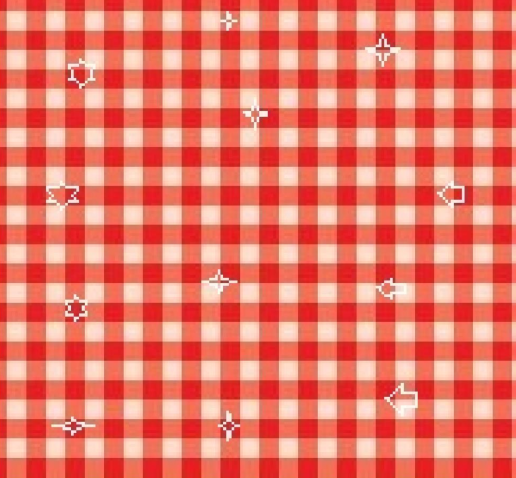
\includegraphics[scale=0.55]{../figures/test-4.png}
    	\quad
    	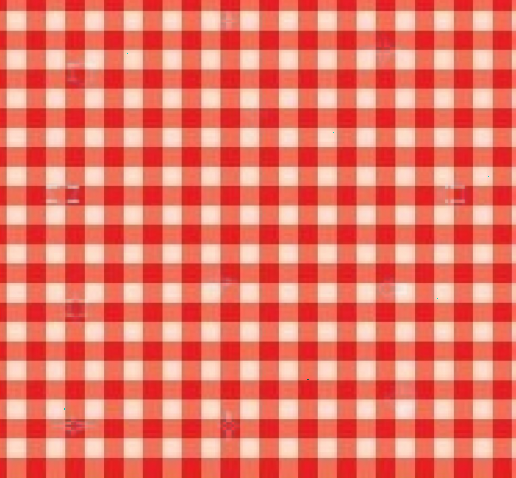
\includegraphics[scale=0.276]{../figures/A-4.png}
    	\quad
    	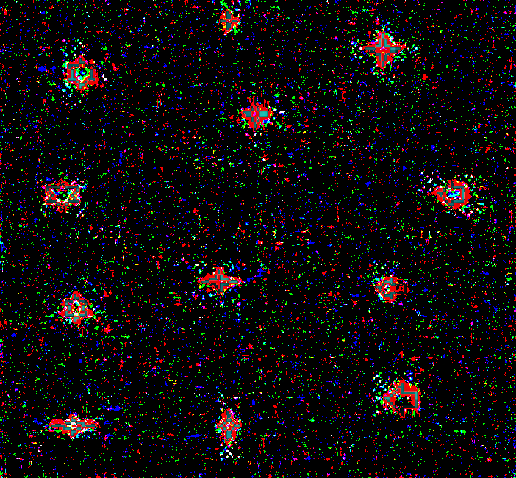
\includegraphics[scale=0.276]{../figures/E-4.png}
    	\caption{从左到右:原图、恢复图、残差图}
    \end{figure}
    \begin{figure}[h]
    	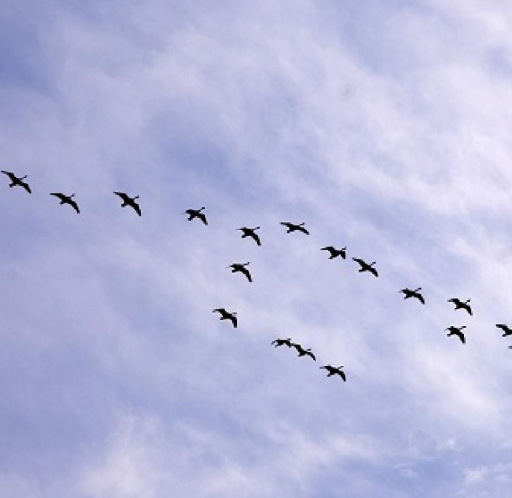
\includegraphics[scale=0.55]{../figures/test-6.png}
    	\quad
    	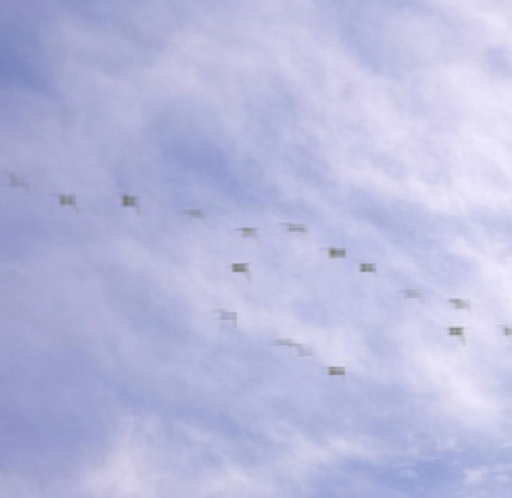
\includegraphics[scale=0.276]{../figures/A-5.png}
    	\quad
    	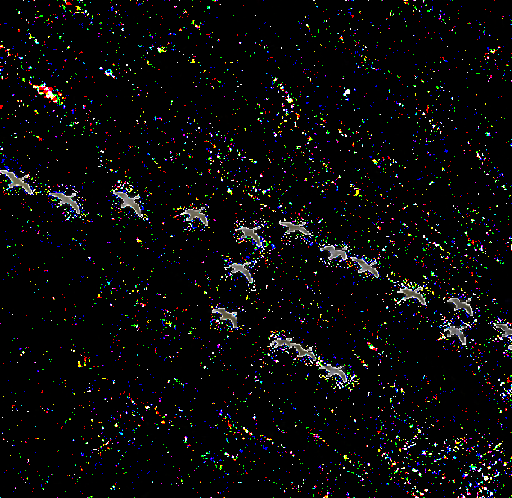
\includegraphics[scale=0.276]{../figures/E-5.png}
    	\caption{从左到右:原图、恢复图、残差图}
    \end{figure}
    \clearpage
    \begin{figure}[h]
    	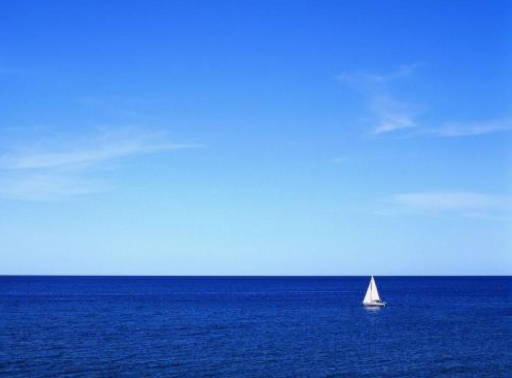
\includegraphics[scale=0.56]{../figures/test-7.png}
    	\quad
    	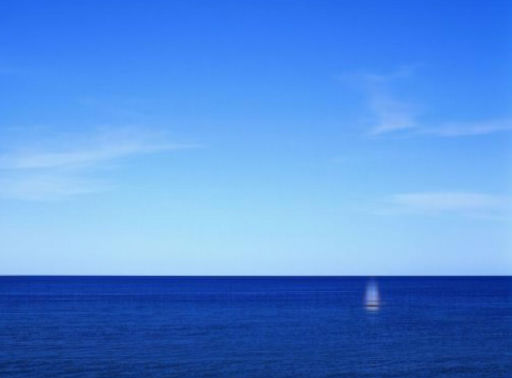
\includegraphics[scale=0.28]{../figures/A-0.png}
    	\quad
    	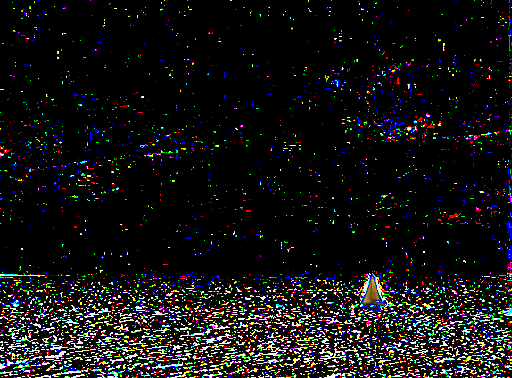
\includegraphics[scale=0.28]{../figures/E-0.png}
    	\caption{从左到右:原图、恢复图、残差图}
    \end{figure}
    
    \begin{figure}[h]
    	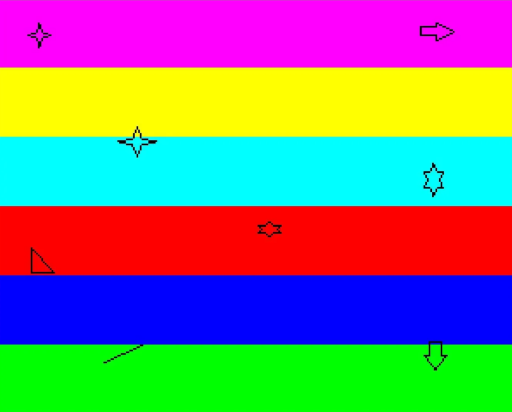
\includegraphics[scale=0.56]{../figures/test-1.png}
    	\quad
    	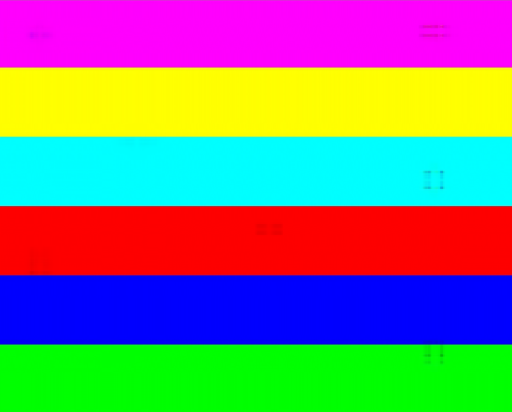
\includegraphics[scale=0.28]{../figures/A-6.png}
    	\quad
    	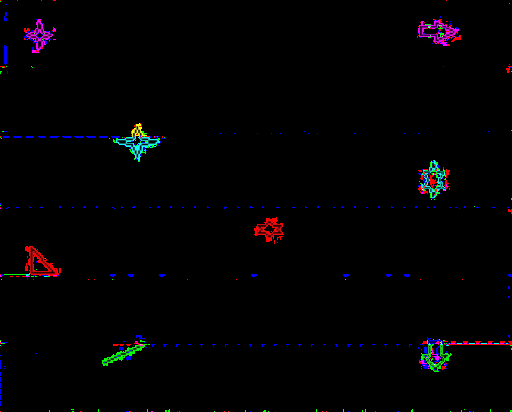
\includegraphics[scale=0.28]{../figures/E-6.png}
    	\caption{从左到右:原图、恢复图、残差图}
    \end{figure}
     
    \subsection{结果对比}
    \begin{figure}[h]
    	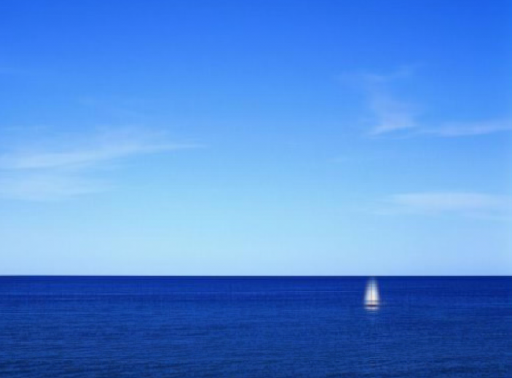
\includegraphics[scale=0.28]{../figures/A-2.png}
    	\quad
    	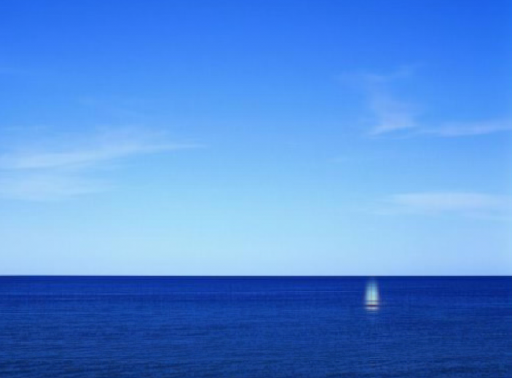
\includegraphics[scale=0.28]{../figures/A-3.png}
    	\quad
    	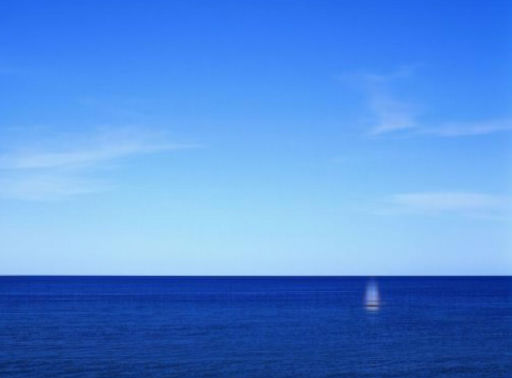
\includegraphics[scale=0.28]{../figures/A-0.png}
    	\caption{从左往右内循环的最大迭代次数分别为1000,3000,4500}
    \end{figure}

 \setcounter{section}{8}
\section*{\centerline{八、结论与解释}}
\setcounter{subsection}{0} 

\subsection{结论一}
    效果分析:通过效果图可以发现,我们的算法对于图像颜色简单、纹理清晰明了、有一定规律的图像分离效果非常明显。恢复图中几乎完全看不出原来“噪声”的存在。比如图1和图4,图像相对简单,低秩分离效果非常好,恢复图中几乎没有白边图案。然而对于复杂度相对较高的图像,我们发现效果比前者稍逊,比如对于图2中的恢复图,我们可以明显发现大雁没有完全被剔除留下的灰色痕迹,还有图3中恢复图中帆船没有完全被剔除留下的微弱痕迹。其实上述情况我们可以用直观理解,因为图像简单某种程度上就暗示着理想的恢复图的秩就非常低,而我们模型假设中就默认了理想恢复图就应该满足低秩条件。图像复杂度越低,低秩条件满足程度越高,我们得到的结果理论更好。

\subsection{结论二}
	循环最大迭代次数的影响:对于精确ADMM算法,在不断增大内循环最大迭代次数,我们可以发现图像恢复效果逐渐变好,这在结果对比中的图5可以体现:随着内循环最大迭代次数增大,帆船的身影逐渐在慢慢被海的颜色所覆盖。事实上,笔者构建的精确ADMM算法某种程度上也是不精确的,这是因为设定的内循环最大迭代次数大多数情况会截断内循环的迭代,所以设置的内循环最大迭代次数越大,内循环收敛程度越佳,效果进而越好。这就可以解释为什么没有内循环的不精确ADMM算法效果不尽人意,因为理论上没有内循环的ADMM算法为内循环最大迭代次数为1的精确ADMM算法。对于外循环最大迭代次数其实对结果并没有太大影响,因为外循环的损失下降很快,往往还没有达到最大迭代次数就已经达到设定的tol以内。

\subsection{结论三}
	我们着重关注残差图(噪声图),我们可以发现三个通道分别得到的残差位置并没有完全重合,但是重合集中的地方可以发现就是"噪声"所在位置。这里笔者要解释为什么残差图中噪声和原图像颜色并不总是一致,这是因为在分解成A和E矩阵之后,残差矩阵E中可能会出现负值,在将其转化成图像的时候我们需要使用Uint8进行数据类型转化,这时负数的像素点就会进行取模256的操作,导致噪声颜色并不一定和原图像相同。

 \setcounter{section}{9}
\section*{\centerline{九、问题}}
\setcounter{subsection}{0} 
    其实主要的问题是时间效率和结果效果不能均衡的问题,如果内循环次数越少,我们得到的算法结果越差,然而对于512×512图像,如果设置内循环最大迭代次数为3000,算法运行时间就可能达到20min。能否存在一种低秩分解更好算法做到对于图像恢复效果和速度兼顾的效果。由于时间、精力因素,笔者无法进行深入研究。

\bibliographystyle{ieeetr}
\bibliography{refer}

\end{document}
